\section{K-means}

\mode<presentation>{
\begin{frame} 
    \begin{center} \huge
        \secname
    \end{center}
    \begin{center}
		points within a region $\Longrightarrow$ cluster
    \end{center}
\end{frame}
}

\begin{frame}
K-means is simple.
\end{frame}

\begin{frame}{Finding structure in the data}

\begin{center}
\slidesonly{
	\includegraphics<1>[width=6cm]{img/clustering_no-color_no-labels_2p}
	\includegraphics<2>[width=6cm]{img/clustering_no-color_no-labels_4p}
	\includegraphics<3>[width=6cm]{img/clustering_no-color_no-labels}
	}
	\includegraphics<4->[width=6cm]{img/clustering_color}
	\notesonly{
	\captionof{figure}{Example clustering of 2D points into M=2 clusters}
	}
\end{center}


\slidesonly{
\visible<5>{
\begin{itemize}
\item proximity must count for something
\item Points that fall within a region form a cluster
\item Points within a cluster have more in common with one another than points from different clusters
\end{itemize}
}
}

\end{frame}

\subsubsection{In plain English}

\begin{frame}{Finding structure in the data}

\notesonly{
Data is observed. We want to be able to describe some ``structure'' in the data.
We base our approach on something very simple and intuitive: 
A set of 
objects (points) that share common features tend to fall in some region. A second set of objects that also share common features but which are different from the first set fall in another region.
This ``structure'' we are describing groups, ``clusters'' a collection of points based on their proximity to a region.  
A point that is further away from this collection and closer to another is grouped with the points associated with that other region. 
We do have to decide on how many clusters we think exist in a dataset.
}

\question{What does clustering give us?}
 
\begin{itemize}
\item[-] Instead of describing each point by its absolute location, we will be able to describe it by the cluster it is assigned to.
\begin{equation}
\text{point}~\vec x \in \R^N \quad \longrightarrow \quad~\text{cluster index}~q \in \N
\end{equation} 
\item We will be able to describe the entire dataset by the partitions we've found that separate the clusters.
\item We'll draw relations between simple clustering and other algorithms (embedding algorithms, density estimation)
\end{itemize}

\end{frame}

\begin{frame}{K-means is simple}

\underline{Problem}\\

Group the dataset $\left\{ \vec x^{(1)}, \vec x^{(2)}, \ldots, \vec x^{(p)} \right\}$, where $\vec x \in \R^N$, into $M$ clusters\notesonly{\footnote{$M$ is actually equivalent to the $K$ in $K$-means.}}.

\slidesonly{
\begin{center}
	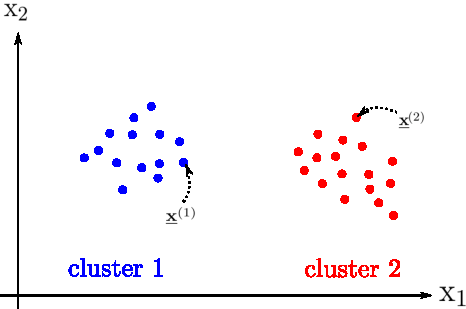
\includegraphics[width=6cm]{img/clustering_color}
\end{center}
}

\end{frame}

\begin{frame}{Formalizing K-means}

\only<1-3>{

\notesonly{
\underline{The K-means approach}:\\
}

Determine $M$ ``good'' prototypes $\vec w_1, \ldots, \vec w_M \in \R^N$ and \only<3>{\underline}{assign} each data point $\vec x^{(\alpha)}$ to the prototype closest to it.\\
}

\slidesonly{
\begin{center}
	\includegraphics<1>[width=6cm]{img/clustering_color}
	\includegraphics<2>[width=6cm]{img/clustering_color_proto}
\end{center}
	}

\end{frame}

\begin{frame}{Formalizing K-means: Assignment variables}

\begin{center}
	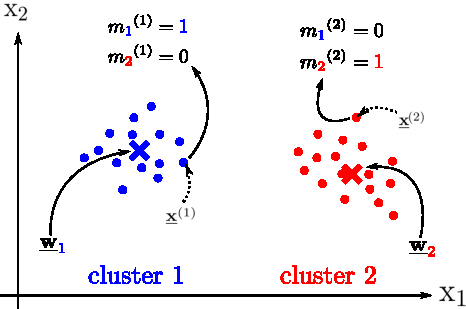
\includegraphics[width=6cm]{img/clustering_color_proto_assignment}
	\notesonly{
	\captionof{figure}{Example clustering of 2D points into M=2 clusters with location of cluster prototypes (centroids)}
	}
\end{center}
	
\notesonly{
The assignment is formalized by introducing the following} assignment variable $m_q^{(\alpha)}$ for each point $\alpha$ and each cluster $q$:

\begin{equation}
\label{eq:assignment}
	m_q^{(\alpha)} := \left\{ \begin{array}{ll}
		1, & \text{if } \vec{x}^{(\alpha)} \text{ belongs to cluster } q
		\\\\
		0, & \text{otherwise}
	\end{array} \right. 
\end{equation}

\notesonly{$q$ is used as the cluster index. We have a total of $p \cdot M$ assignment variables for a dataset with $p$ points and choice of number of clusters $M$.}

\end{frame}

\begin{frame}{Formalizing K-means: Assignment variables}

\slidesonly{Cluster $p$ points into $M$ clusters $\leadsto$ $p\cdot M$ assignment variables}

\pause

$m_q^{(\alpha)}$ is a binary variable and with the normalization:

\begin{equation}
    \label{eq:assignmentnormalization}
	\sum\limits_q m_q^{(\alpha)} = 1,
\end{equation}
we limit the assignment of each point to only one cluster. We refer to this as a ``hard'' assignment\footnote{This will be relaxed when we talk about ``soft'' K-means.}.

\end{frame}

\begin{frame}{The K-means cost function}

A solution to our problem is one that
\begin{enumerate}
\item finds the location of the prototypes $\vec w_q$ and 
\item assigns all points 
\end{enumerate}
such that they are optimal in terms of \slidesonly{``cost''}\notesonly{the following cost}
\pause
which measures the average distance between a prototype and the subset of points assigned to it:

\begin{align}
\label{eq:kmeanscost}
E_{ \big[ \big\{ m_q^{(\alpha)} \big\}, \big\{ \vec{w}_q \big\} 
		\big] }^T &= \frac{1}{p} \sum\limits_{q,\alpha} m_q^{(\alpha)}
		\big( \vec{x}^{(\alpha)} - \vec{w}_q \big)^2\\
        &= \frac{1}{p} \sum_{\alpha=1}^{p} \sum_{q=1}^{M} m_q^{(\alpha)}
		\big( \vec{x}^{(\alpha)} - \vec{w}_q \big)^2 \eqexcl \underset{\big\{ m_q^{(\alpha)} \big\}, \big\{ \vec{w}_q \big\}}{\min}
\end{align}

\notesonly{
When we consider the definition of $m_q^{(\alpha)}$ as \emph{binary variables} as provided by \eqref{eq:assignment} and their normalization as in \eqref{eq:assignmentnormalization}, we realize that for each point $\alpha$ only one of its $m_q^{(\alpha)}$ is non-zero (and =1). Therefore, we are effectively evaluating the distance $\big( \vec{x}^{(\alpha)} - \vec{w}_q \big)^2$ only \textbf{once} for that point $\alpha$, namely it's distance only to the one cluster $q$ that point is assigned to.

This simplifies our expression for the cost function:


}
\begin{align}
\label{eq:kmeanscostsimple}
E_{ \big[ \big\{ m_q^{(\alpha)} \big\}, \big\{ \vec{w}_q \big\} 
		\big] }^T 
        &= \frac{1}{p} \sum_{\alpha=1}^{p}
		\big( \vec{x}^{(\alpha)} - \vec{w}_q \big)^2 \eqexcl \underset{\big\{ m_q^{(\alpha)} \big\}, \big\{ \vec{w}_q \big\}}{\min}
\end{align}


\notesonly
{
Where the cost is minimized over the set of discrete variables $\big\{ m_q^{(\alpha)} \big\}$ as well as the set of continuous variables $\big\{ \vec{w}_q \big\}$.

Minimizing the average distance between each prototype $\vec w_q$ and the points assigned to it leads to partitioning the data into $M$ clusters such that a point is assigned to a cluster $q$ because it is closest to $\vec w_q$.
}

\end{frame}

